\documentclass[a4paper, 12pt]{article}

\usepackage{exercise-sheet}
\usepackage{global-macros}
\usepackage{biblatex}
\usepackage{csquotes}
\addbibresource{../bib/bibliografia.bib}
\usepackage{graphicx}
\graphicspath{{../fig/}}
\usepackage{hyperref}
\hypersetup{
    colorlinks=true,
    linkcolor=blue,
    filecolor=magenta,
    urlcolor=cyan,
    pdfpagemode=FullScreen,
}

%% Packages

\usepackage{mathtools, amsthm}

%% Environments

\theoremstyle{plain} % default
\newtheorem{teo}{Teorema}[section]
\newtheorem*{teo*}{Teorema}
\newtheorem{lem}{Lema}[section]
\newtheorem*{lem*}{Lema}
\newtheorem{prop}{Proposição}
\newtheorem*{prop*}{Proposição}
\newtheorem{cor}[teo]{Corolário}
\newtheorem*{axiom}{Axioma}

\newtheorem*{TAU}{Teorema da Aproximação Universal}
\newtheorem*{Riesz}{Teorema da Representação de Riesz}

\theoremstyle{definition}
\newtheorem{defn}{Definição}
\newtheorem{conj}{Conjectura}[section]
\newtheorem{exmp}{Exemplo}[section]
\newtheorem{rem}{Observação}[section]
\newtheorem*{rem*}{Observação}

\theoremstyle{remark}
\newtheorem*{note}{Nota}
\newtheorem{case}{Caso}


% Macros


\DeclarePairedDelimiter{\dotprod}{\langle}{\rangle}

\DeclareMathOperator{\rk}{rk}
\DeclareMathOperator{\intt}{int}
\DeclareMathOperator{\diam}{diam}
\DeclareMathOperator{\rref}{rref}
\DeclareMathOperator{\vspan}{span}
\DeclareMathOperator{\proj}{proj}
\DeclareMathOperator{\lin}{Lin}
\DeclareMathOperator{\supp}{supp}

\DeclareMathOperator{\posto}{posto}

% Swap the definition of \abs* and \norm*, so that \abs
% and \norm resizes the size of the brackets, and the 
% starred version does not.

\newcommand{\transpose}{\mathsf{T}}

%% Multiline comments
\newcommand{\comment}[1]{}


\title{Um estudo elementar sobre as curvas \emph{Geodésicas}}
\author{Caio Lins}
\date{\today}

\begin{document}

\maketitle

\tableofcontents

\section{Introdução}

Neste trabalho, vamos definir o conceito de geodésica e estudar suas propriedades mais elementares, culminando com a demonstração de sua existência e unicidade.
A exposição foi integralmente baseada no capítulo 4 de \cite{ronaldo}.
Apesar de não chegarmos a abordar esta parte, é importante enfatizar que o interesse sobre geodésicas vem do fato de que, \emph{localmente}, elas minimizam o comprimento de caminhos entre pontos na superfície.
Isso poderá ser visualizado quando mostrarmos alguns exemplos de geodésicas.
Antes de tudo, porém, vamos apenas revisar um pouco da notação, bem como um teorema, que serão utilizados.

Denotamos o produto vetorial entre dois vetores \( v, w \in \R^{ 3 } \) por \( v \times w \).
A esfera unitária em \( \R^{ 3 } \), isto é, o conjunto \( ( x, y, z ) \in \R^{ 3 } : x^2 + y^2 + z^2 = 1 \) será denotada por \( \mathbb{S}^2 \).
Quando escrevermos, por exemplo, \( t \mapsto t^2 \), estaremos fazendo referência à \emph{função} que mapeia um número \( t \) ao número \( t^2 \).
Além disso, dada uma função \( f \), a notação \( f \equiv 0 \) significa que \( f \) é \emph{identicamente nula}, ou seja, \( f ( x ) = 0 \) para todo \( x \) no domínio de \( f \).
Por fim, relembramos o enunciado do teorema que garante a existência e unicidade das soluções de uma equação diferencial ordinária:
\begin{teo*}
    Seja \( D \subseteq \R \times \R^{ n } \) um retângulo fechado com \( ( t_{ 0 }, u_{ 0 } ) \in D \).
    Seja \( f : D \to \R^{ n } \) uma função contínua em \( t \) e Lipschitz contínua em \( y \).
    Então, existe \( \varepsilon > 0 \) tal que a equação
    \begin{equation*}
        y' ( t ) = f ( t, y ( t ) )
    ,\end{equation*}
    junto com a restrição \( y ( t_{ 0 } ) = y_{ 0 } \) tem uma solução única no intervalo \( ( t_{ 0 } - \varepsilon, t_{ 0 } + \varepsilon ) \).
\end{teo*}


%% \( \times \)
%% \( \mathbb{S}^{ n } \)
%% EG - F^2 > 0
%% \( x \mapsto f ( x ) \)
%% \( f \equiv 0 \)

\section{Isometrias}

Quando estamos trabalhando com aplicações de \( \R^{ n } \) em \( \R^{ m } \), isometrias são aquelas que preservam o comprimento de vetores.
Ao mudar o ambiente de trabalho para superfícies, a definição de isometria faz referência à derivada da aplição e, consequentemente, aos espaços tangentes a essas superfícies.
Mais explicitamente, temos:
\begin{defn}[Isometria]
    Dadas superfícies regulares \( S_{ 1 } \) e \( S_{ 2 } \), dizemos que uma aplicação \( f : S_{ 1 } \to S_{ 2 } \) é uma \emph{isometria} se é um difeomorfismo e, para todo \( p \in S_{ 1 } \) e todos \( w, v \in T_{ p } S_{ 1 } \) temos
    \begin{equation}
        \dotprod{ df_{ p } w, df_{ p } v } = \dotprod{ w, v }
        \label{eq: isometria}
    .\end{equation}
    Ainda, dizemos que \( f : S_{ 1 } \to S_{ 2 } \) é uma \emph{isometria local} se, para todo \( p \in S_{ 1 } \) existem abertos \( V_{ 1 } \subseteq S_{ 1 } \) e \( V_{ 2 } \subseteq V_{ 2 } \), tais que \( p \in V_{ 1 }, f ( p ) \in V_{ 2 } \) e \( f \mid_{ V_{ 1 } } : V_{ 1 } \to V_{ 2 } \) é uma isometria.

Finalmente, duas superfícies regulares são ditas \emph{isométricas} se existe uma isometria entre elas.
\end{defn}

Agora, alguns comentários.
Observe que, se \( f \) é isometria local e difeomorfismo, então é isometria.
Também perceba que, pela \emph{identidade de polarização}:
\begin{equation*}
    \dotprod{ w, v } = \frac{ \norm{ w + v }^2 - \norm{ w - v }^2 }{ 4 }
\end{equation*}
a condição (\ref{eq: isometria}) é equivalente a termos
\begin{equation}
    \norm{ df_{ p }w } = \norm{ w }
    \label{eq: isometria2}
\end{equation}
para todo \( w \in T_{ p } S_{ 1 } \).

Observe, ainda, que se \( f : S_{ 1 } \to S_{ 2 } \) cumpre (\ref{eq: isometria2}) (ou, equivalentemente, (\ref{eq: isometria}), pelo que acabamos de mostrar), então, para todo \( p \in S_{ 1 } \), temos que \( df_{ p } \) é um isomorfismo.
De fato, a injetividade vem do fato de que se \( df_{ p }w = df_{ p }v \), então
\begin{equation*}
    \norm{ w - v } = \norm{ df_{ p } ( w - v ) } = \norm{ df_{ p }w - df_{ p }v } = 0
,\end{equation*}
de modo que \( w = v \).
Agora, como \( 2 = \dim T_{ f ( p ) } S_{ 2 } \geq \dim df_{ p } ( T_{ p } S_{ 1 } ) = 2 \), necessariamente temos \( T_{ f ( p ) } S_{ 2 } = df_{ p } ( T_{ p } S_{ 1 } ) \), ou seja, \( df_{ p } \) é sobrejetiva.
Dessa forma, pelo Teorema da Função Inversa, para cada \( p \in S_{ 1 } \) existem vizinhanças \( V_{ 1 } \ni p \) e \( V_{ 2 } \ni f ( p ) \) em \( S_{ 1 } \) e \( S_{ 2 } \), respectivamente, tais que \( f\mid_{ V_{ 1 } } : V_{ 1 } \to V_{ 2 } \) é difeomorfismo.
Ou seja, \( f \) é isometria local.

Com isso, provamos a seguinte proposição, que caracteriza as isometrias locais.
\begin{prop}
    Uma aplicação entre superfícies regulares é uma isometria local se, e somente se, preserva a primeira forma fundamental.
\end{prop}

Dado esse resultado, podemos esperar que isometrias locais preservem, de uma certa forma, os coeficientes da primeira forma fundamental.
Isso de fato ocorre, como podemos ver na seguinte proposição:

\begin{prop}
    Sejam \( S_{ 1 } \) e \( S_{ 2 } \) superfícies regulares, \( f : S_{ 1 } \to S_{ 2 } \) uma isometria local e \( X : U \subseteq \R^{ 2 } \to S_{ 1 } \) uma parametrização local de \( S_{ 1 } \), cuja imagem \( X ( U ) \defeq V \) é um aberto de \( S_{ 1 } \) tal que \( f \mid_{ V } : V \to f ( V ) \subseteq S_{ 2 } \) é uma isometria.
    Sob essas hipóteses, \( Y = f \circ X : U \to S^{ 2 } \) é uma parametrização local de \( S_{ 2 } \), cujos coeficientes da primeira forma fundamental coincidem com aqueles da parametrização \( X \).
    \label{conserva primeira forma}
\end{prop}

\begin{proof}
    Como a composição de difeomorfismos é um difeomorfismo e tanto \( f \mid_{ V } \) quanto \( X \) são difeomorfismos, temos que \( Y \) é uma parametrização local de \( S_{ 2 } \).
    Além disso, como a restrição de \( f \) a \( V \) é uma isometria, temos, para todo \( ( u, v ) \in U \):
    \begin{align*}
        \dotprod{ Y_{ u } ( u, v ), Y_{ u } ( u, v ) }
        &= \dotprod{
            ( f \circ X )_{ u } ( u, v ),
            ( f \circ X )_{ u } ( u, v )
        } \\
        &= \dotprod{
            df_{ X ( u, v ) } X_{ u } ( u, v ),
            df_{ X ( u, v ) } X_{ u } ( u, v )
        } \\
        &= \dotprod{ 
            X_{ u } ( u, v ), X_{ u } ( u, v )
        }
    .\end{align*}
    Ou seja, o coeficiente \( E \) da primeira forma fundamental é preservado.
    Analogamente demonstra-se que
    \begin{equation*}
        \dotprod{ Y_{ u }, Y_{ v } } = \dotprod{ X_{ u }, X_{ v } }
        \ \text{ e } \
        \dotprod{ Y_{ v }, Y_{ v } } = \dotprod{ X_{ v }, X_{ v } }
    .\end{equation*}
    Com isso, todos os coeficientes da primeira forma fundamental são preservados, como queríamos demonstrar.
\end{proof}

\section{Geodésicas}

\begin{defn}
    Uma curva parametrizada diferenciável em uma superfície regular \( S \), \( \gamma : I \subseteq \R \to S \), é dita uma \emph{geodésica parametrizada} se seu vetor aceleração é sempre perpendicular ao espaço tangente da superfície, ou seja, se para todo \( p = \gamma ( t ) \in \gamma ( I ) \) temos \( \gamma'' ( t ) \in \left\{ T_{ \gamma ( t ) } S \right\}^{ \perp } \).
    Analogamente, uma curva regular \( C \subset S \) é dita uma \emph{geodésica} de \( S \) se, para todo ponto \( p \in C \), existe uma parametrização local \( \gamma : I \subseteq \R \to C \), de \( C \) em \( p \), tal que \( \gamma \) é uma geodésica parametrizada.

\comment{
    norma do vetor velocidade da geodesica é constante
    caracterização com produto interno da aceleracao e a normal de gauss *
    equacoes diferenciais
    existencia e unicidade *
    invariancia por isometrias locais
    homogeneidade
}
    
\end{defn}


\section{Exemplos de Geodésicas}

Para ilustrar o conceito de geodésica, vamos exibi-las em algumas superfícies diferentes.

\subsection{Cilindro}

Para encontrar as geodésicas de um cilindro, utilizaremos a Proposição \ref{nao varia por isometria} e obte-las-emos por meio das geodésicas do plano.
Intuitivamente, está claro que as geodésicas em um plano são justamente os segmentos de reta nele contidos.
Para formalizar essa intuição, basta perceber que, dado um desses segmentos de retas, podemos facilmente parametrizá-lo localmente por uma curva de velocidade constante.
Com isso, sua aceleração é nula e, assim, perpendicular ao espaço tangente do plano em cada ponto.

Com esse conhecimento em mãos, pela Proposição \ref{nao varia por isometria} precisamos apenas de encontrar uma isometria entre o plano e o cilindro.
Felizmente, isso não é muito difícil, pois a parametrização usual do cilindro é uma isometria.

Denotando por \( C \defeq \mathbb{S}^{ 1 } \times \R = \left\{ ( x, y, z ) \in \R^{ 3 } : x^2 + y^2 = 1 \right\} \) o cilindro, por \( S \) o plano em \( \R^{ 3 } \) correspondente a \( z = 0 \) e por \( U \defeq \left\{ ( x, y, 0 ) \in S : - \pi < x < \pi \right\} \) o retângulo entre \( -\pi \) e \( \pi \), nossa isometria é \( f : U \subseteq S \to f ( U ) \subseteq C \) dada por
\begin{equation*}
    f ( x, y, z ) = ( \cos x, \sen x, y )
.\end{equation*}

Logo, as geodésicas no cilindro são as imagens de segmentos de reta por \( f \).
Ilustramos algumas delas na Figura \ref{geodesicas cilindro}.

\begin{figure}[htb]
    \begin{center}
        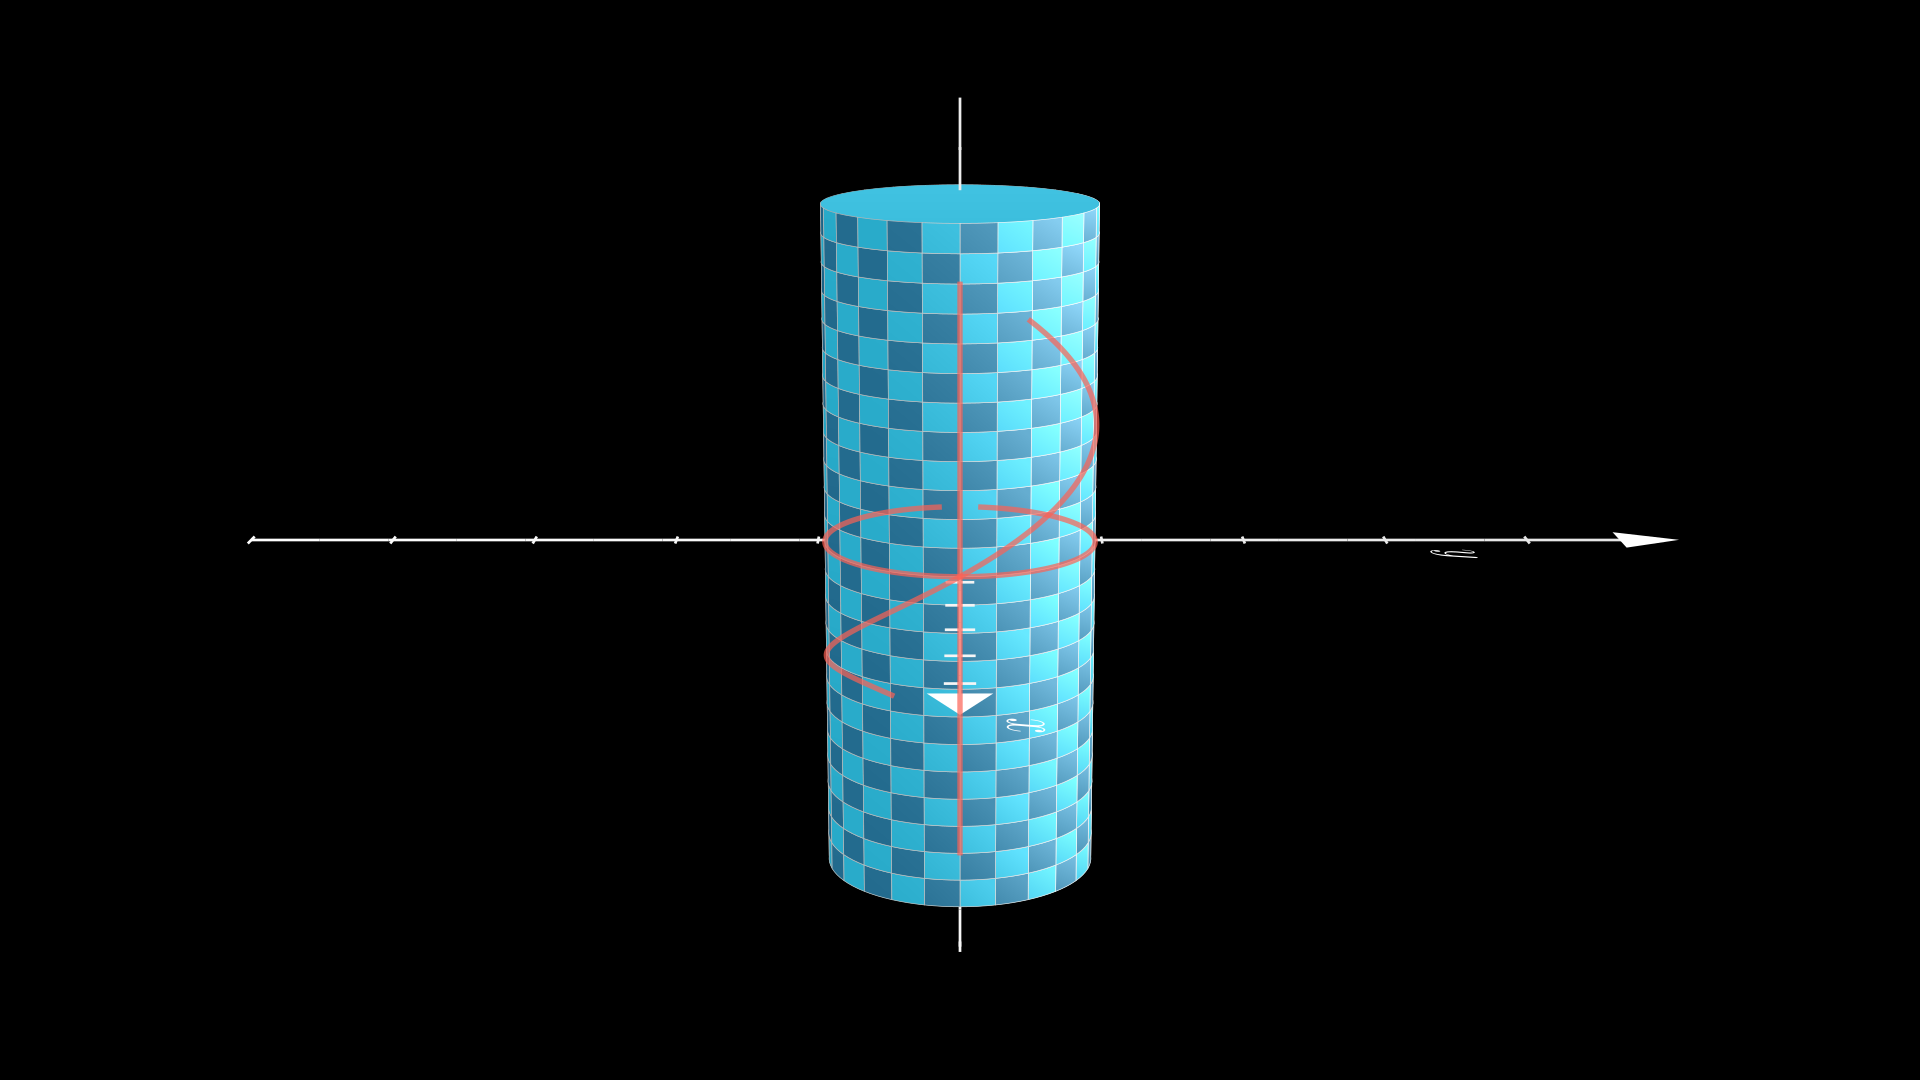
\includegraphics[width=.5\textwidth]{cilindro-1}
        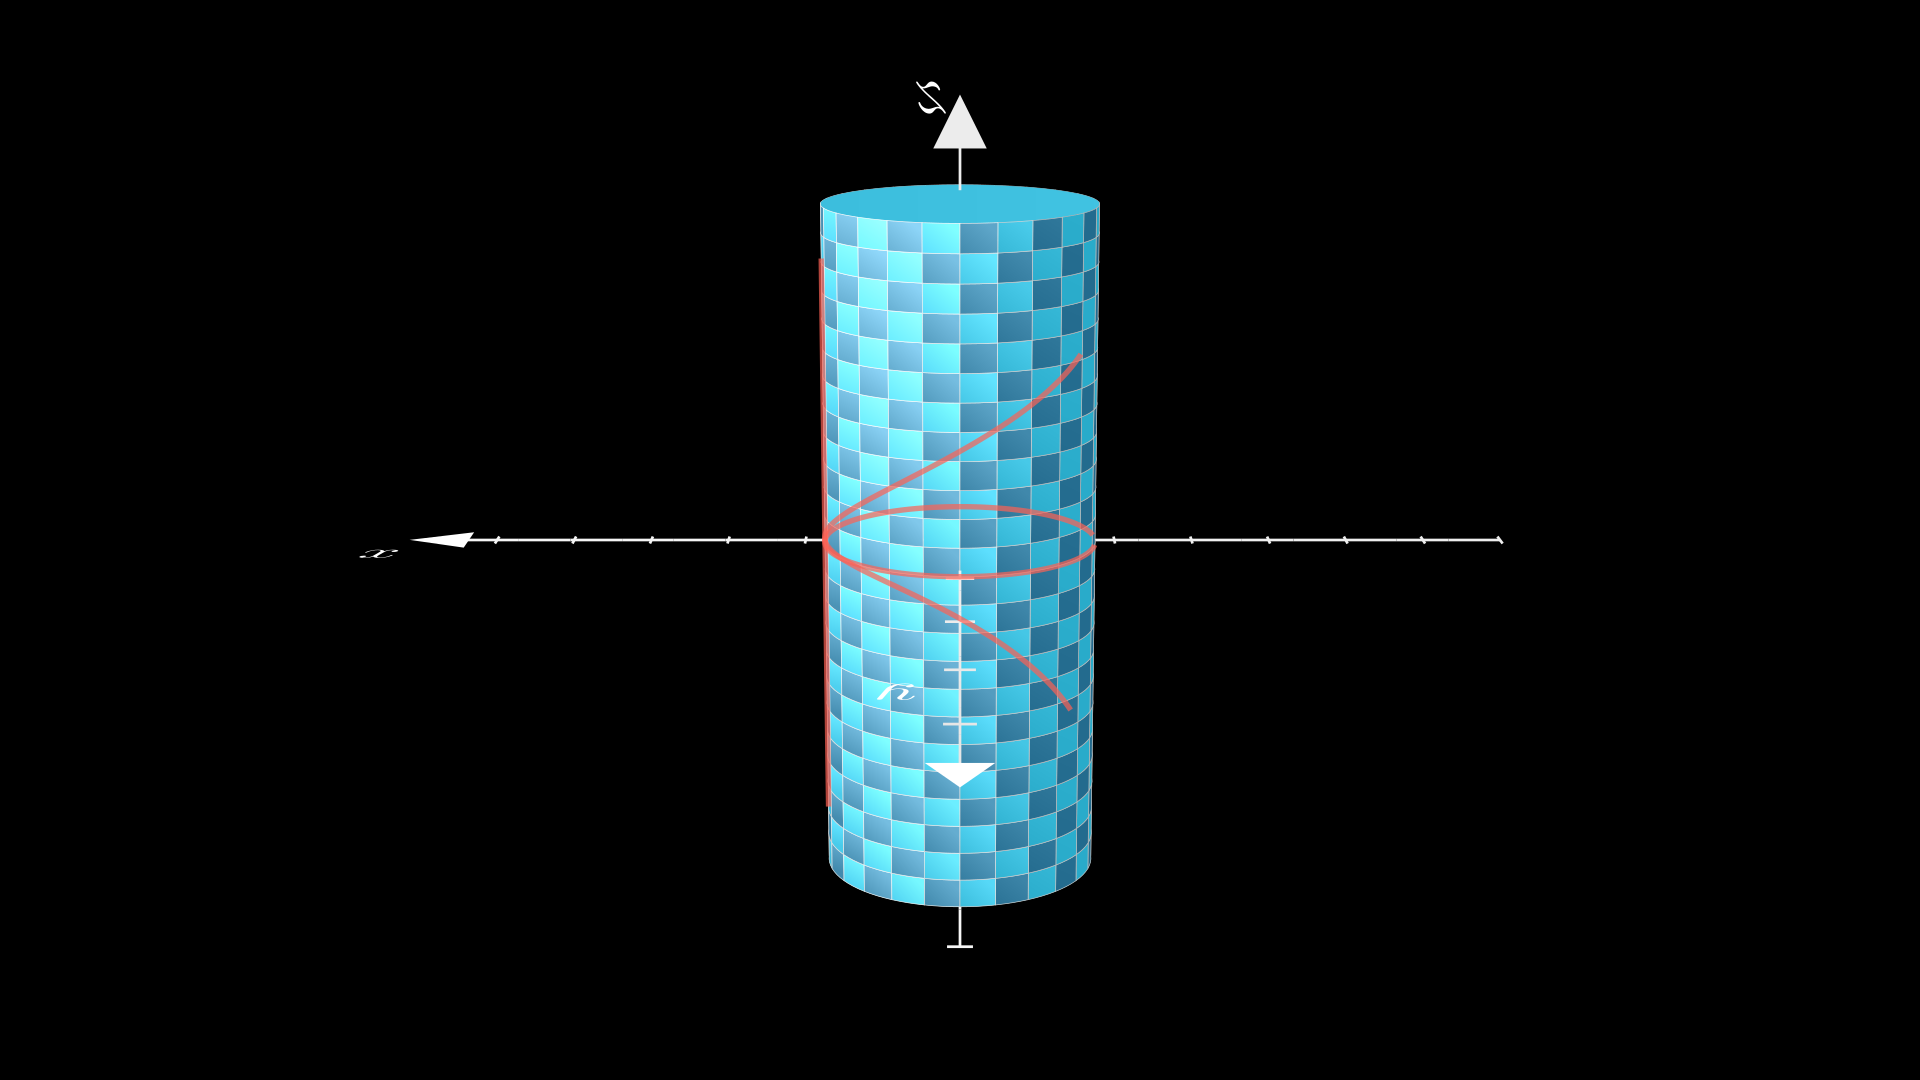
\includegraphics[width=.5\textwidth]{cilindro-2}
        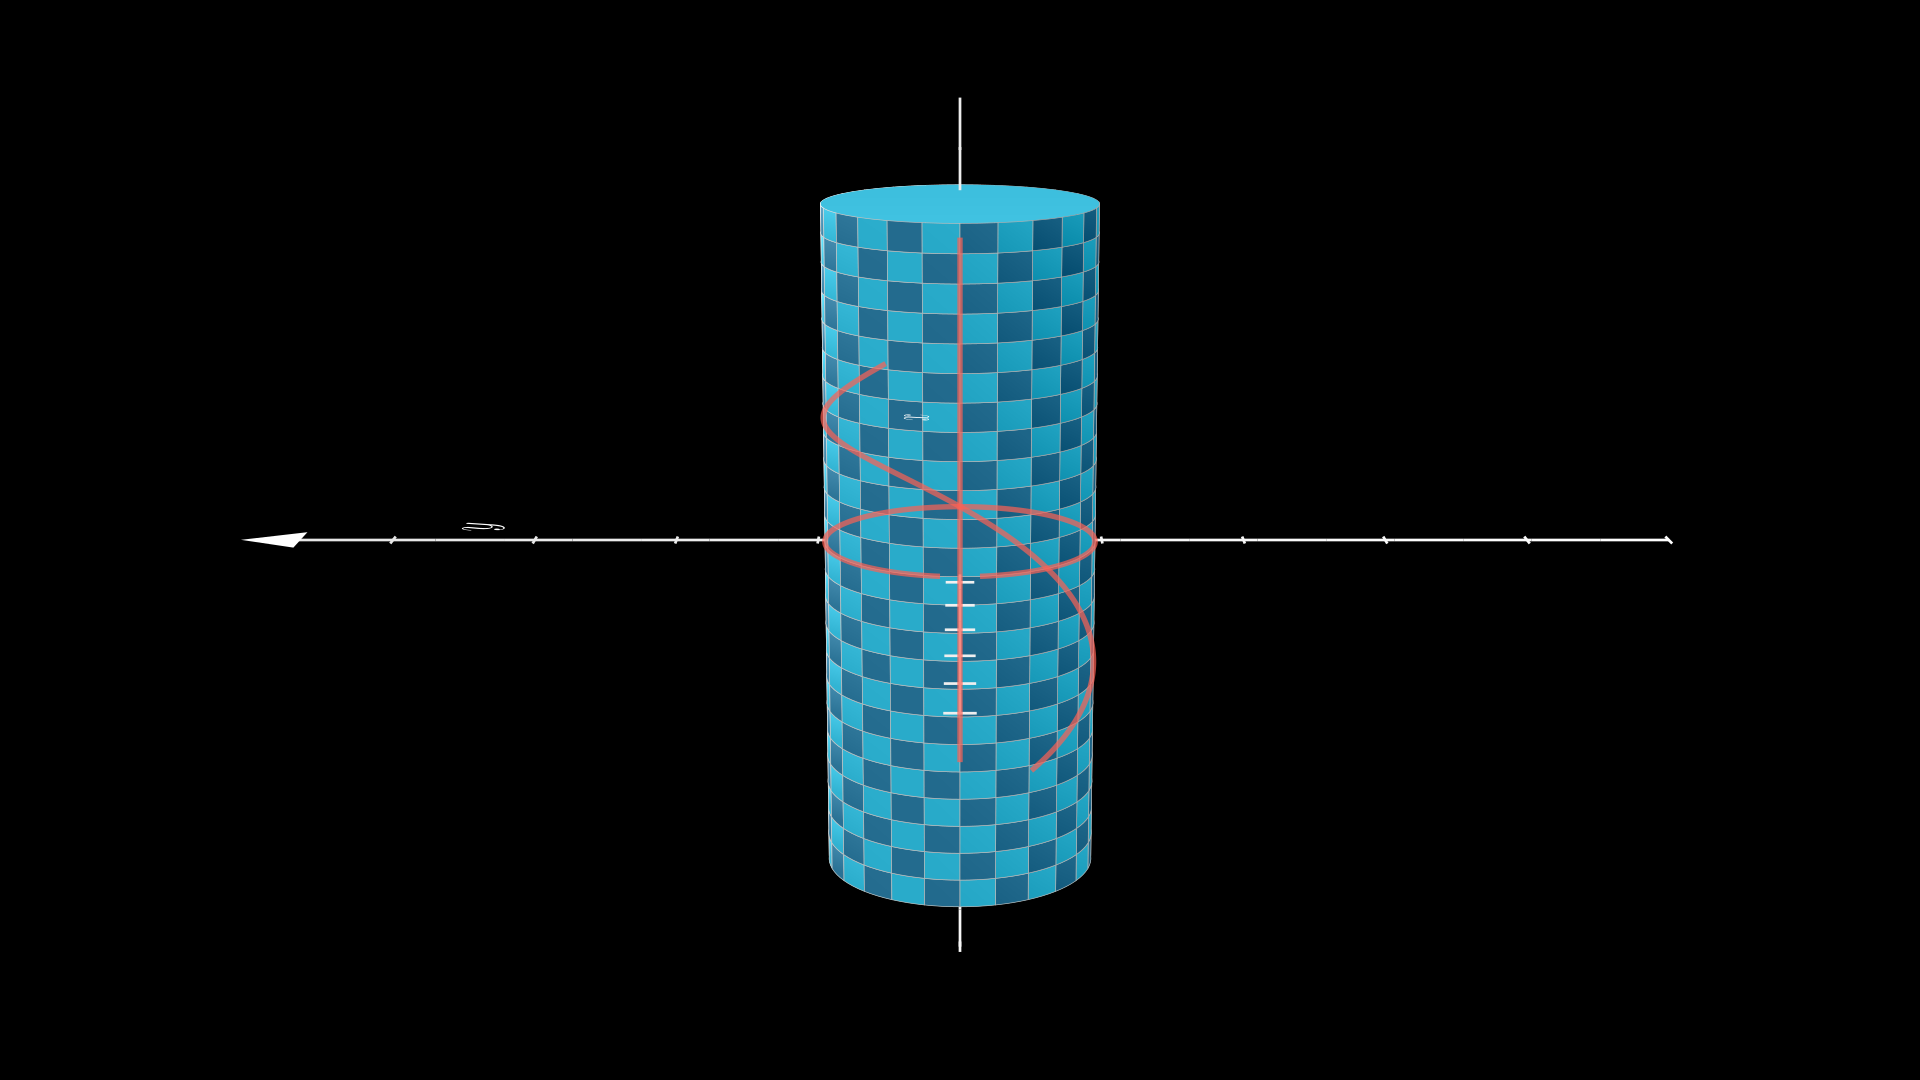
\includegraphics[width=.5\textwidth]{cilindro-3}
        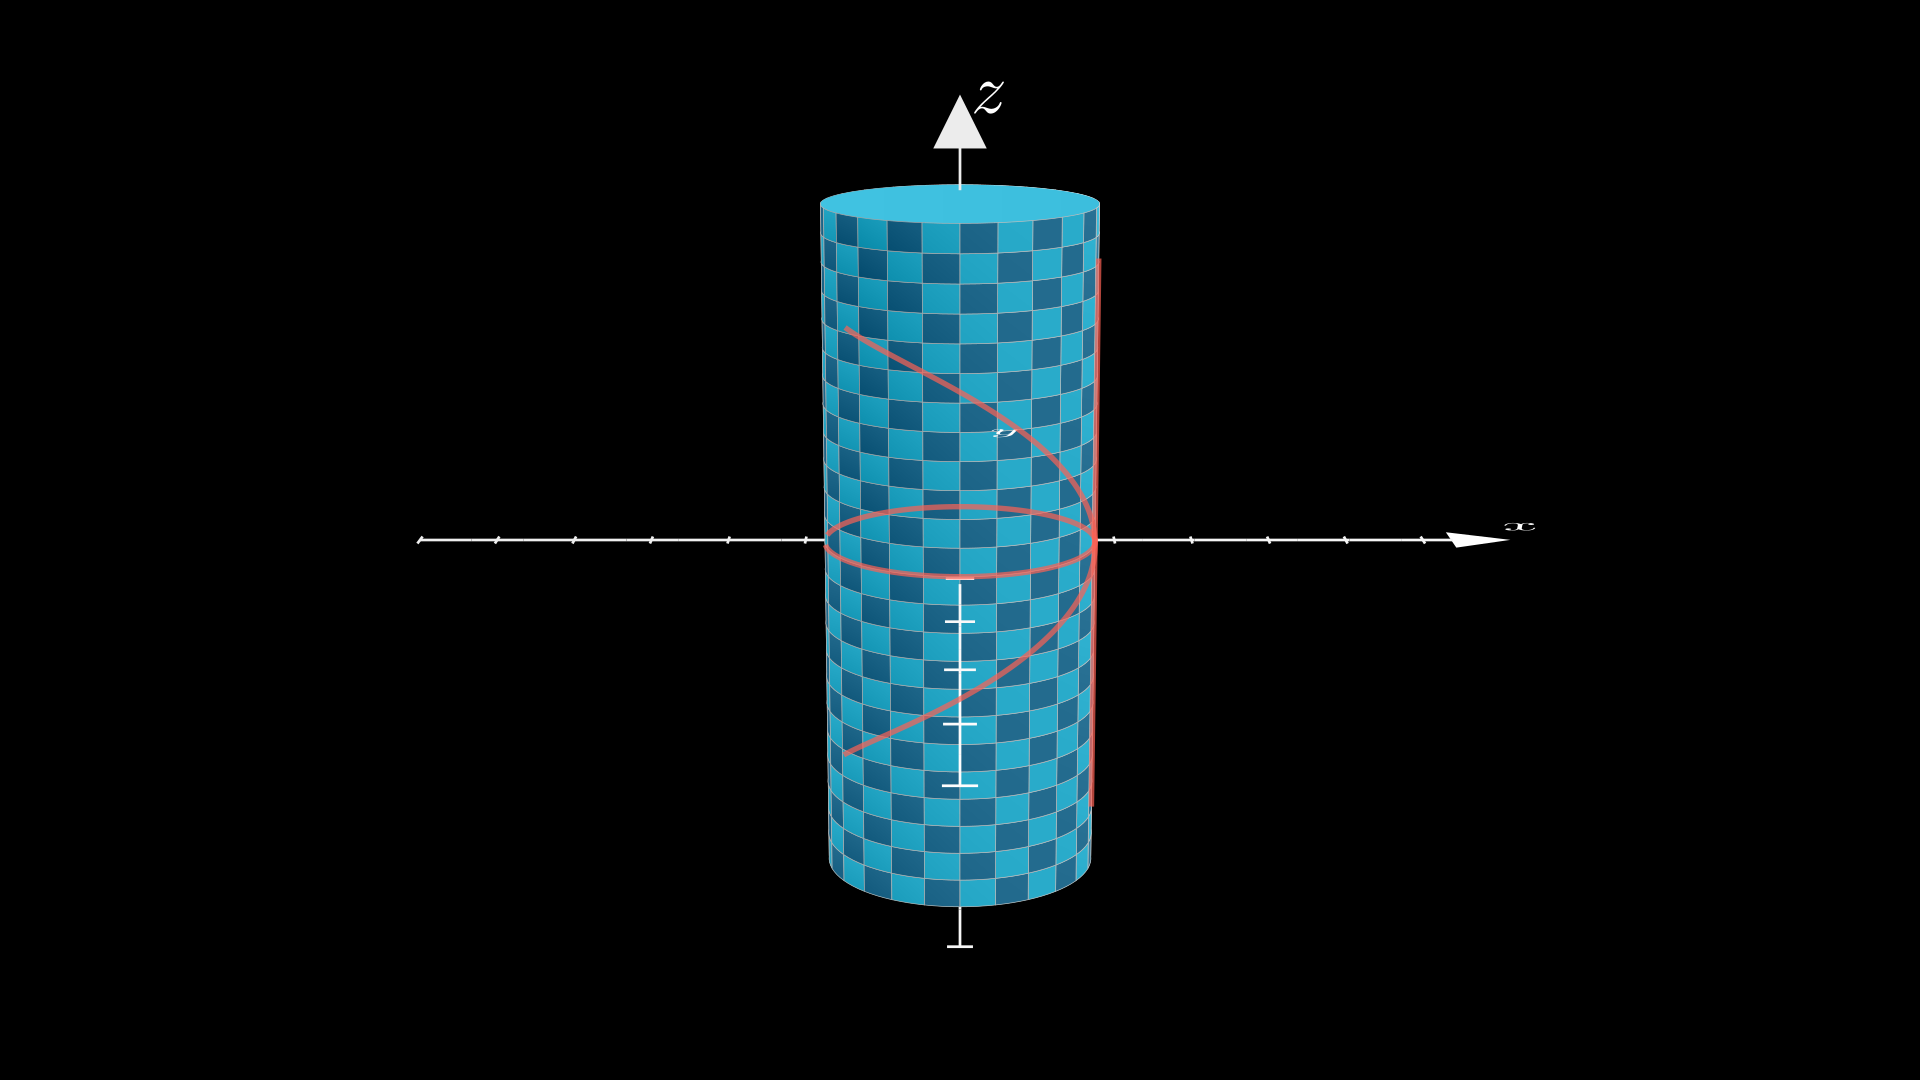
\includegraphics[width=.5\textwidth]{cilindro-4}
    \end{center}
    \caption{Três tipos de geodésicas no cilindro, sob diferentes pontos de vista.}
    \label{geodesicas cilindro}
\end{figure}

\subsection{Esfera}

Para encontrar as geodésicas da esfera, podemos resolver o sistema de equações diferenciais apresentado em (\ref{difeq}), ou podemos prosseguir por um argumento mais geométrico, como a seguir.
Primeiramente, perceba que o grande arco \( C \) de \( \mathbb{S}^{ 2 } \) parametrizado por \( \gamma ( \theta ) = ( \cos ( \theta ), \sen ( \theta ), 0 ) \) tem aceleração \( \gamma'' ( \theta ) = - ( \cos ( \theta ), \sen ( \theta ) ) = - \gamma ( \theta ) \).
Como \( T_{ \gamma ( t ) } \mathbb{S}^{ 2 } = \left\{ \gamma ( t ) \right\}^{ \perp } \), temos que \( \gamma'' ( t ) \) é perpendicular ao espaço tangente em \( \gamma ( t ) \) para todo \( t \).
Logo, \( \gamma ( t ) \) descreve uma geodésica na esfera.
Agora, como todo grande arco de \( \mathbb{S}^{ 2 } \) é a imagem de \( C \) por uma rotação (a qual, por ser uma transformação linear ortogonal, é isometria), concluímos da Proposição \ref{nao varia por isometria} concluímos que todo grande arco de \( \mathbb{S}^{ 2 } \) é uma geodésica.
Alguns deles estão representados na Figura \ref{geodesicas esfera}.

\begin{figure}[htb]
    \begin{center}
        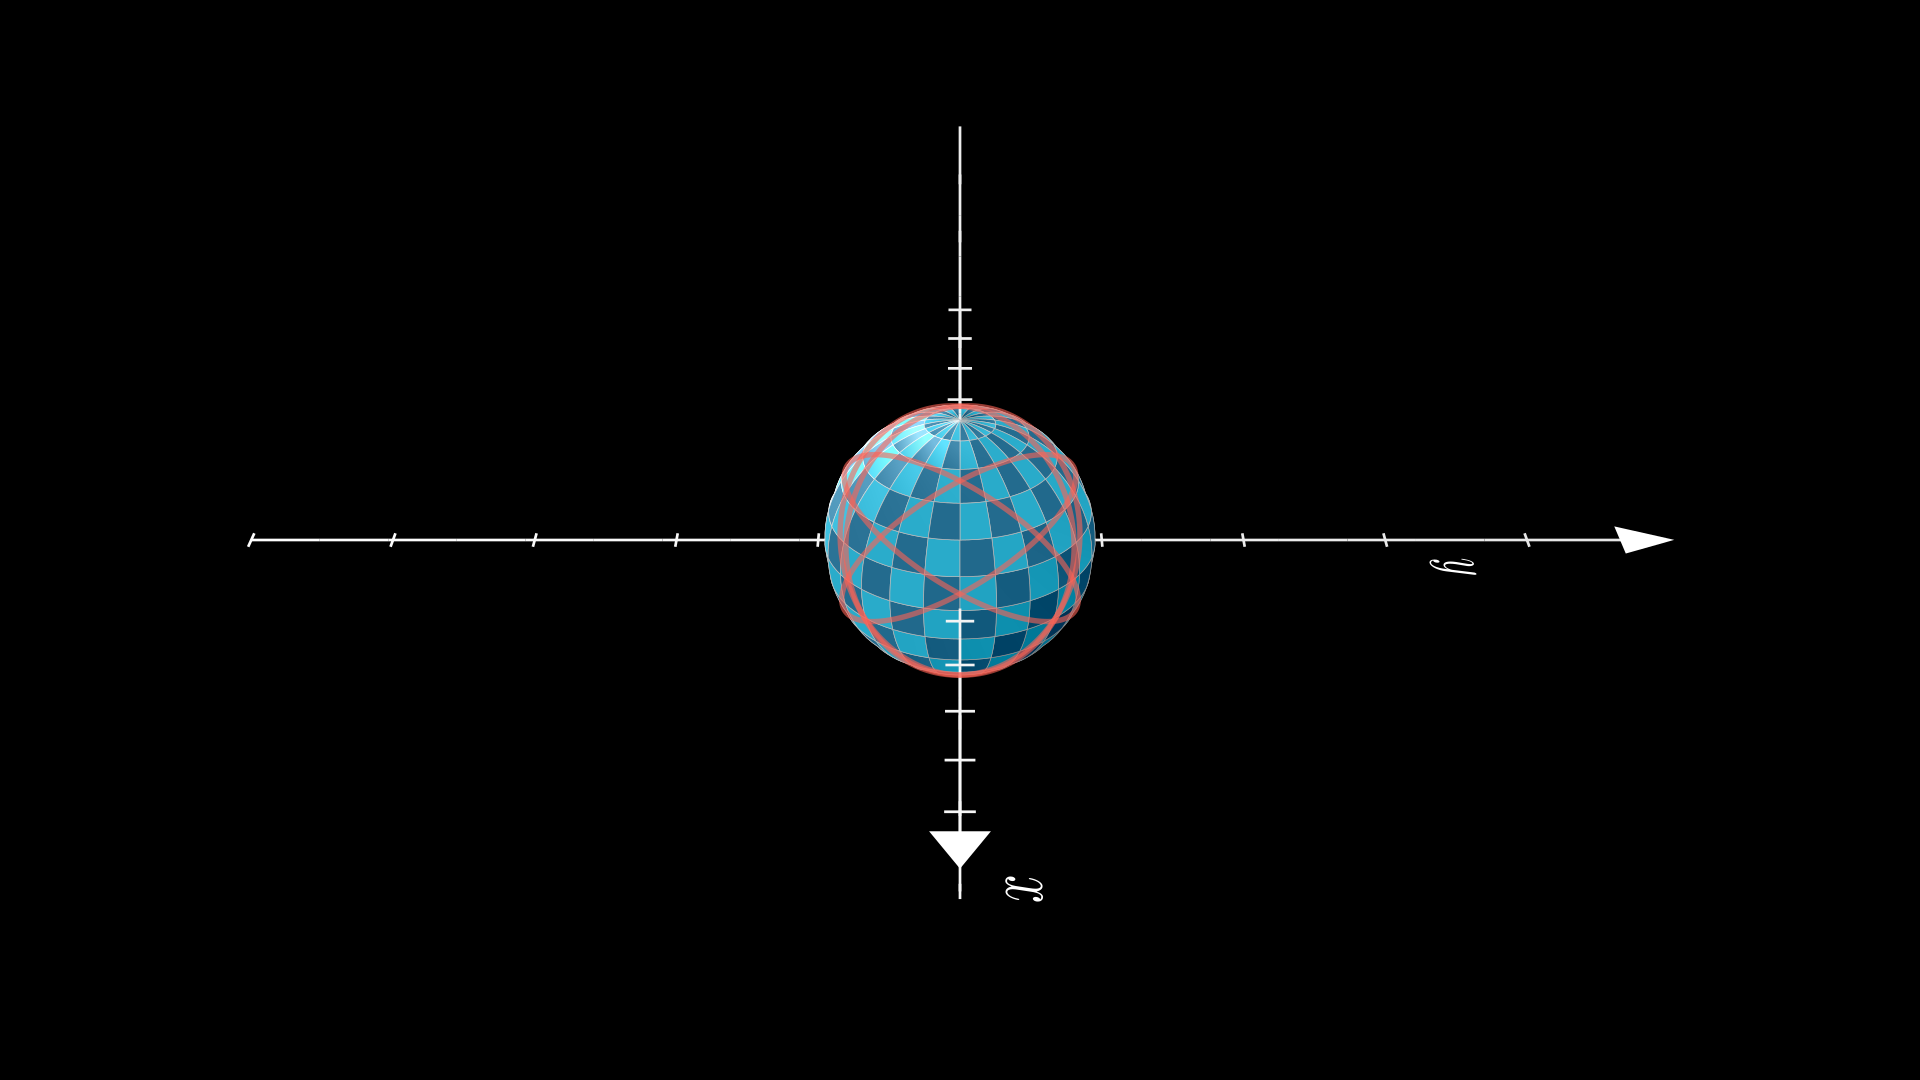
\includegraphics[width=.7\textwidth]{esfera-1}
        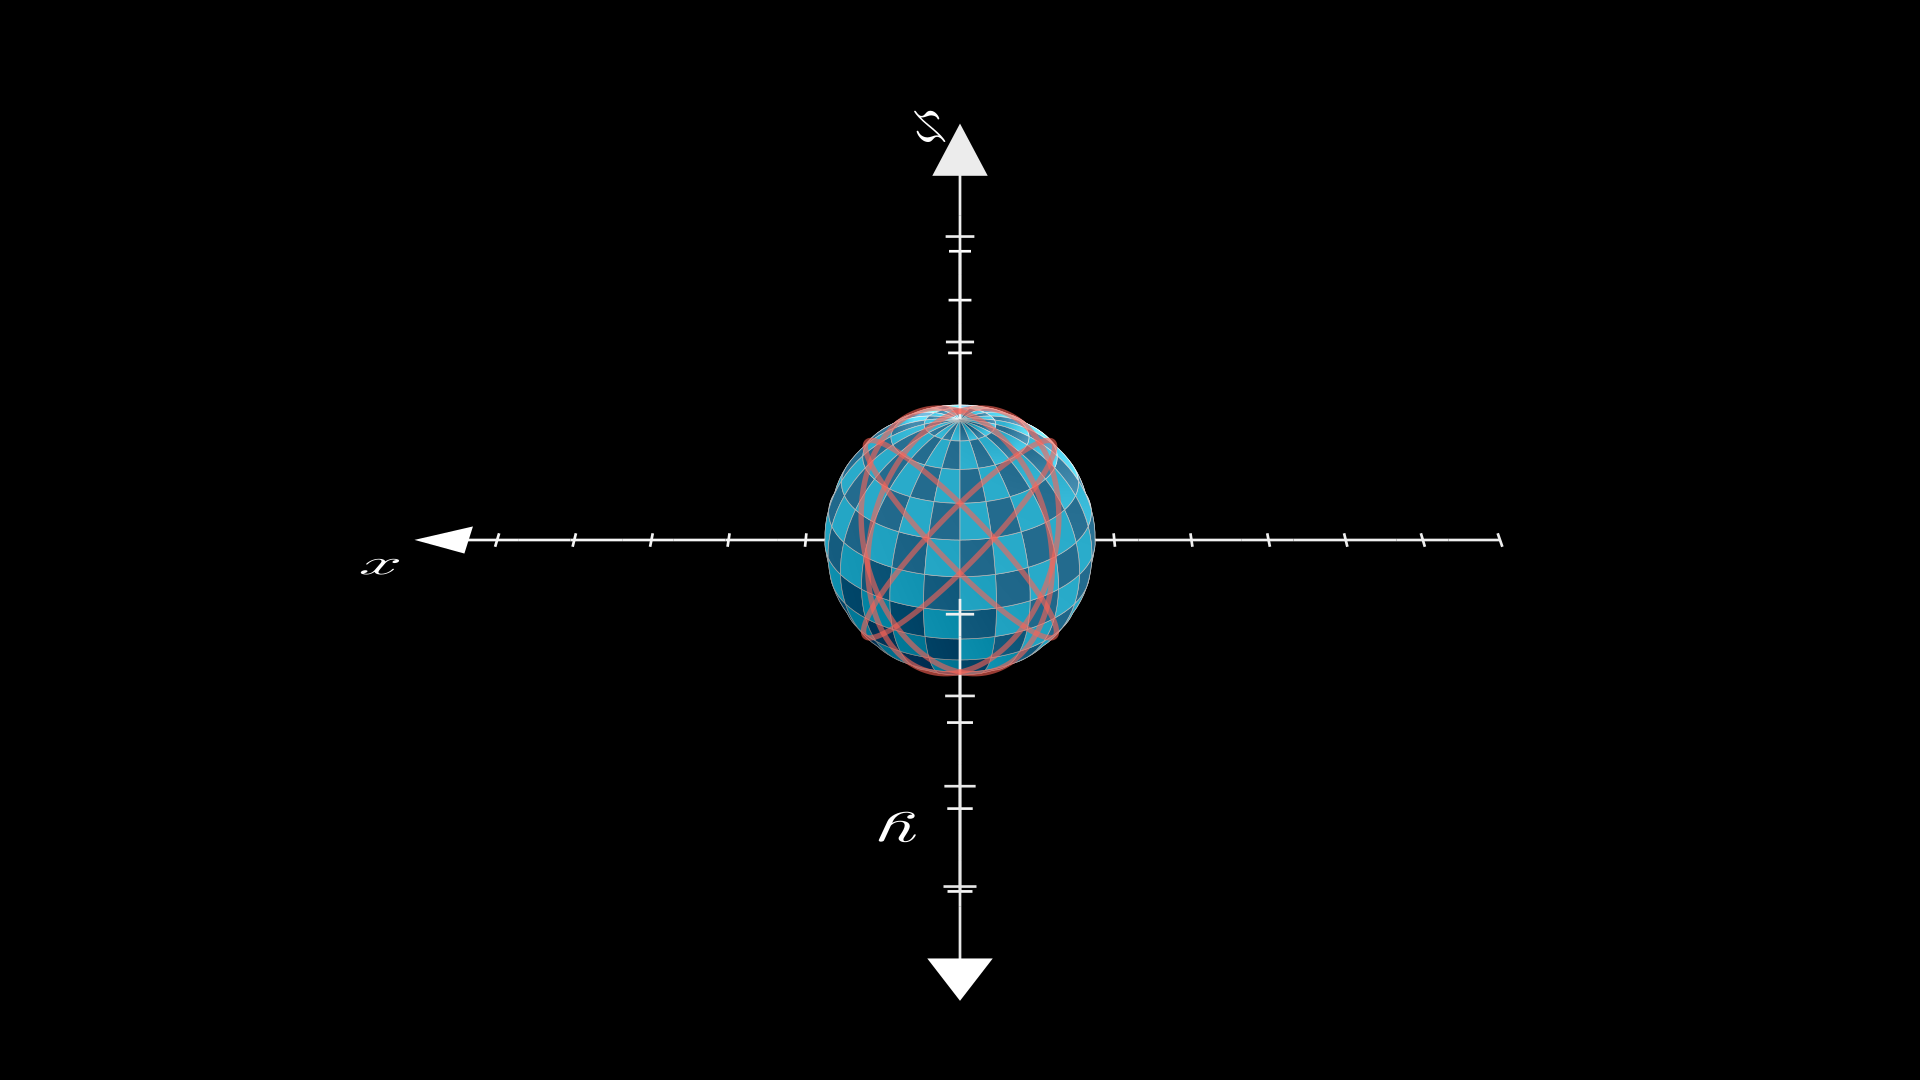
\includegraphics[width=.7\textwidth]{esfera-2}
    \end{center}
    \caption{Alguns grandes arcos em \( \mathbb{S}^{ 2 } \), sob dois pontos de vista.}
    \label{geodesicas esfera}
\end{figure}

\section{Conclusão}

Neste trabalho, introduzimos o conceito de geodésica e demonstramos suas propriedades mais elementares, culminando com a demonstração de sua existência e unicidade em superfícies regulares.
Um próximo passo bastante evidente é demonstrar que geodésicas de fato minimizam distâncias sobre a superfície, pelo menos localmente, e, reciprocamente, que caminhos que minimizam distâncias são geodésicas.


\printbibliography

\end{document}
